% Architecture diagram of the SEN421 right-sizing experiment.
% Compile on its own:  pdflatex architecture.tex  ->  architecture.pdf
\documentclass[tikz,border=4pt]{standalone}
\usepackage[scaled=0.92]{helvet}
\renewcommand{\familydefault}{\sfdefault}
\usetikzlibrary{positioning,shapes.symbols,arrows.meta,calc}
\definecolor{hz}{HTML}{D50C2D}
\definecolor{netblue}{HTML}{257DE0}
\definecolor{netfill}{HTML}{EEF5FF}
\definecolor{ink}{HTML}{191919}
\definecolor{ink2}{HTML}{666666}
\definecolor{notefill}{HTML}{FFFBE6}
\definecolor{notedraw}{HTML}{B38600}
\begin{document}
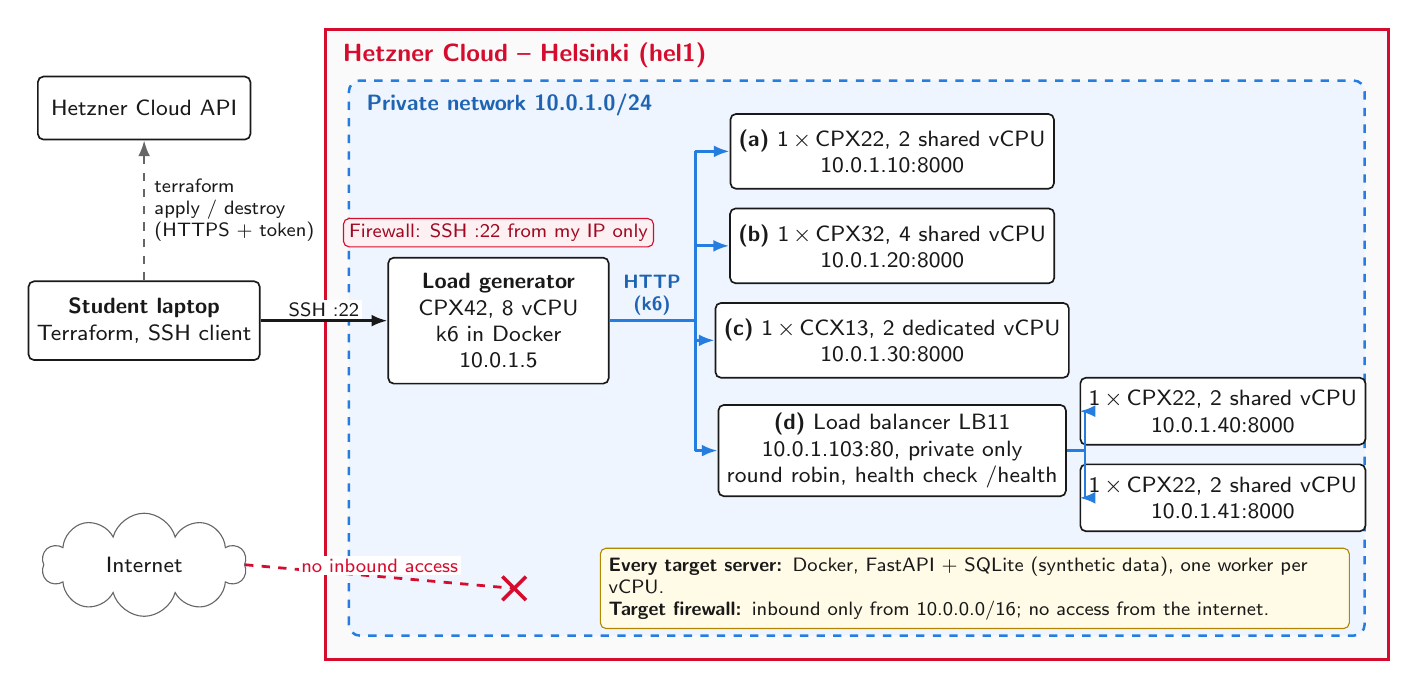
\begin{tikzpicture}[
  font=\footnotesize, text=ink,
  box/.style={draw=ink, rounded corners=2pt, fill=white, align=center, inner sep=3pt, line width=0.6pt},
  target/.style={box, minimum width=4.0cm, minimum height=0.95cm},
  fw/.style={draw=hz, rounded corners=2pt, fill=hz!6, text=hz!75!black, font=\scriptsize, inner sep=2pt},
  http/.style={-{Latex[length=2mm]}, draw=netblue, line width=1pt},
  ssh/.style={-{Latex[length=2mm]}, draw=ink, line width=1pt},
  api/.style={-{Latex[length=2mm]}, draw=ink2, dashed, line width=0.8pt},
]
% --- regions -------------------------------------------------------------
\draw[hz, line width=1.2pt, fill=black!2] (3.8,-0.1) rectangle (17.3,7.9);
\node[anchor=north west, text=hz, font=\small\bfseries] at (3.9,7.85) {Hetzner Cloud -- Helsinki (hel1)};
\draw[netblue, dashed, line width=0.9pt, fill=netfill, rounded corners=4pt] (4.1,0.2) rectangle (17.0,7.25);
\node[anchor=north west, text=netblue!80!black, font=\footnotesize\bfseries] at (4.2,7.2) {Private network 10.0.1.0/24};

% --- outside Hetzner ------------------------------------------------------
\node[box, minimum width=2.7cm, minimum height=0.8cm] (api) at (1.5,6.9) {Hetzner Cloud API};
\node[box, minimum width=2.7cm, minimum height=1.0cm] (pc) at (1.5,4.2) {\textbf{Student laptop}\\Terraform, SSH client};
\node[cloud, draw=ink2, cloud puffs=10, aspect=1.8, minimum width=2.6cm, minimum height=1.3cm, align=center] (inet) at (1.5,1.1) {Internet};

% --- load generator --------------------------------------------------------
\node[box, minimum width=2.8cm, minimum height=1.6cm] (lg) at (6.0,4.2)
  {\textbf{Load generator}\\CPX42, 8 vCPU\\k6 in Docker\\10.0.1.5};
\node[fw, above=0.12cm of lg] {Firewall: SSH :22 from my IP only};

% --- targets ---------------------------------------------------------------
\node[target] (a) at (11.0,6.35) {\textbf{(a)} 1\,$\times$\,CPX22, 2 shared vCPU\\10.0.1.10:8000};
\node[target] (b) at (11.0,5.15) {\textbf{(b)} 1\,$\times$\,CPX32, 4 shared vCPU\\10.0.1.20:8000};
\node[target] (c) at (11.0,3.95) {\textbf{(c)} 1\,$\times$\,CCX13, 2 dedicated vCPU\\10.0.1.30:8000};
\node[target, minimum height=1.15cm] (lb) at (11.0,2.55) {\textbf{(d)} Load balancer LB11\\10.0.1.103:80, private only\\round robin, health check /health};
\node[box, minimum width=2.9cm, minimum height=0.85cm] (d1) at (15.2,3.05) {1\,$\times$\,CPX22, 2 shared vCPU\\10.0.1.40:8000};
\node[box, minimum width=2.9cm, minimum height=0.85cm] (d2) at (15.2,1.95) {1\,$\times$\,CPX22, 2 shared vCPU\\10.0.1.41:8000};
\node[draw=notedraw, fill=notefill, rounded corners=2pt, align=left, font=\scriptsize, inner sep=3pt, text width=9.3cm] (note) at (12.05,0.8)
  {\textbf{Every target server:} Docker, FastAPI + SQLite (synthetic data), one worker per vCPU.\\
   \textbf{Target firewall:} inbound only from 10.0.0.0/16; no access from the internet.};

% --- traffic -----------------------------------------------------------------
\coordinate (bus) at (8.5,4.2);
\draw[netblue, line width=1pt] (lg.east) -- (bus);
\draw[netblue, line width=1pt] (8.5,2.55) -- (8.5,6.35);
\foreach \t in {a,b,c,lb} { \draw[http] (8.5,0 |- \t.west) -- (\t.west); }
\node[text=netblue!80!black, font=\scriptsize\bfseries, align=center, inner sep=1pt, above] at (7.95,4.22) {HTTP\\(k6)};
\draw[netblue, line width=1pt] (lb.east) -- (13.45,2.55);
\draw[netblue, line width=1pt] (13.45,1.95) -- (13.45,3.05);
\draw[http] (13.45,3.05) -- (d1.west);
\draw[http] (13.45,1.95) -- (d2.west);

% --- management and blocked traffic -----------------------------------------
\draw[ssh] (pc.east) -- node[above, font=\scriptsize, fill=white, inner sep=1pt]{SSH :22} (lg.west);
\draw[api] (pc.north) -- node[right, font=\scriptsize, align=left]{terraform\\apply / destroy\\(HTTPS + token)} (api.south);
\draw[hz, dashed, line width=1pt] (inet.east) -- node[above, font=\scriptsize, text=hz, fill=white, inner sep=1pt]{no inbound access} (note.west -| 6.2,0) coordinate (blk);
\draw[hz, line width=1.3pt] ($(blk)+(-0.15,0.15)$) -- ($(blk)+(0.15,-0.15)$) ($(blk)+(-0.15,-0.15)$) -- ($(blk)+(0.15,0.15)$);
\end{tikzpicture}
\end{document}
